\begin{frame}{Weighted}
\begin{itemize}
\item[$\bullet$]Each interval has a positive weight
\item[$\bullet$]Goal : given $k$ colors, find a coloring maximizing the total weight
\item[$\bullet$]Idea : reducing the problem to a network flow problem (minimum cost flow)
\end{itemize}
\end{frame}

\begin{frame}{From intervals to network}
\begin{itemize}
\item[$\bullet$]Endpoints sorted $\mathrm{x_{1}<x_{2}<\dots<x_{r}}$
\item[$\bullet$]Intervals sorted by increasing right endpoints $\mathrm{I_{1}, I_{2},\dots,  I_{n}}$
\item[$\bullet$]Construction of the network
    \begin{itemize}
    \item Vertices : $\mathrm{s=v_{0},\ \ v_{1},\ \dots, v_{r},\ \ v_{r+1}=t}$
    \item Clique-edges between $\mathrm{(v_{i},v_{i+1})}$ with $\mathrm{cost = 0}$ and $\mathrm{capacity = k}$
    \item Interval-edges between the two endpoints of an interval with $\mathrm{cost = -1 \times weight}$ and $\mathrm{capacity = 1}$
    \end{itemize}
\item[$\bullet$]1 unit of flow = 1 color
\end{itemize}
\end{frame}

\begin{frame}{Example}
\begin{overlayarea}{\textwidth}{\textheight}

\only<1>{
\vspace{0.5cm}
Number of colors = 2
\vspace{0.2cm}

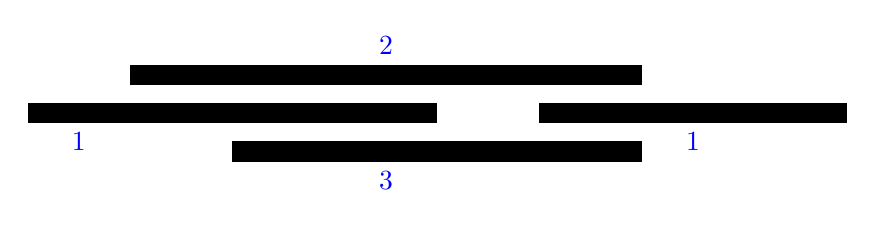
\begin{tikzpicture}[scale=0.65]

\fill (0,0.55) rectangle (8,0.95);
\draw (1, 0.55) node[below]{\textcolor{blue}{$1$}};

\fill (2,1.3) rectangle (12,1.7);
\draw (7, 1.7) node[above]{\textcolor{blue}{$2$}};

\fill (4,-0.2) rectangle (12,0.2);
\draw (7, -0.2) node[below]{\textcolor{blue}{$3$}};

\fill (10,0.55) rectangle (16,0.95);
\draw (13, 0.55) node[below]{\textcolor{blue}{$1$}};
\end{tikzpicture}
}

\only<2>{
\vspace{0.5cm}
Number of colors = 2
\vspace{0.2cm}

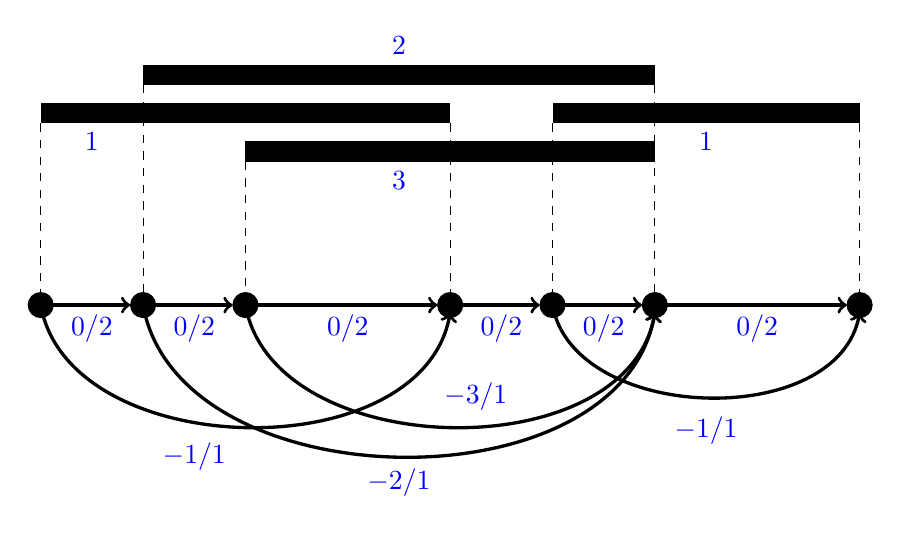
\begin{tikzpicture}[scale=0.65]

\fill (0,0.55) rectangle (8,0.95);
\draw (1, 0.55) node[below]{\textcolor{blue}{$1$}};

\fill (2,1.3) rectangle (12,1.7);
\draw (7, 1.7) node[above]{\textcolor{blue}{$2$}};

\fill (4,-0.2) rectangle (12,0.2);
\draw (7, -0.2) node[below]{\textcolor{blue}{$3$}};

\fill (10,0.55) rectangle (16,0.95);
\draw (13, 0.55) node[below]{\textcolor{blue}{$1$}};

      \foreach \x in {0,2,4,8,10,12,16}
        {\draw (\x,-3) node[fill,circle] {};}

        \draw[dashed] (0,0.55) -- (0,-3);
        \draw[dashed] (2,1.3) -- (2,-3);
        \draw[dashed] (4,-0.2) -- (4,-3);
        \draw[dashed] (8,0.55) -- (8,-3);
        \draw[dashed] (10,0.55) -- (10,-3);
        \draw[dashed] (12,1.3) -- (12,-3);
        \draw[dashed] (16,0.55) -- (16,-3);

        \draw[->,very thick] (0,-3) -- (1.75,-3);
        \draw (1, -3) node[below]{\textcolor{blue}{$0/2$}};
        \draw[->,very thick] (2,-3) -- (3.75,-3);
        \draw (3, -3) node[below]{\textcolor{blue}{$0/2$}};
        \draw[->,very thick] (4,-3) -- (7.75,-3);
        \draw (6, -3) node[below]{\textcolor{blue}{$0/2$}};
        \draw[->,very thick] (8,-3) -- (9.75,-3);
        \draw (9, -3) node[below]{\textcolor{blue}{$0/2$}};
        \draw[->,very thick] (10,-3) -- (11.75,-3);
        \draw (11, -3) node[below]{\textcolor{blue}{$0/2$}};
        \draw[->,very thick] (12,-3) -- (15.75,-3);
        \draw (14, -3) node[below]{\textcolor{blue}{$0/2$}};
        
        
        \draw[->,very thick] (0,-3) to[out=280, in=260] (8,-3.15);
        \draw (3,-5.5) node[below] {\textcolor{blue}{$-1/1$}};
        \draw[->,very thick] (2,-3) to[out=280, in=260] (12,-3.15);
        \draw (7,-6) node[below] {\textcolor{blue}{$-2/1$}};
        \draw[->,very thick] (4,-3) to[out=280, in=260] (12,-3.15);
        \draw (8.5,-5.25) node[above] {\textcolor{blue}{$-3/1$}};
        \draw[->,very thick] (10,-3) to[out=280, in=260] (16,-3.15);
        \draw (13,-5) node[below] {\textcolor{blue}{$-1/1$}};
\end{tikzpicture}
}

\only<3>{
\vspace{0.5cm}
Current flow = \textcolor{blue}{-2} $\Rightarrow$ Current weight =\textcolor{blue}{2}
\vspace{0.2cm}

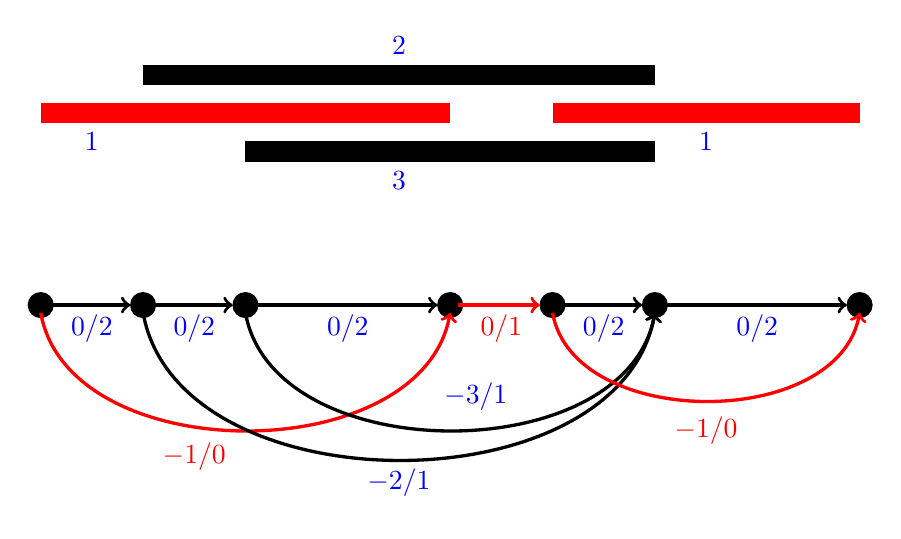
\begin{tikzpicture}[scale=0.65]

\fill[color=red] (0,0.55) rectangle (8,0.95);
\draw (1, 0.55) node[below]{\textcolor{blue}{$1$}};

\fill (2,1.3) rectangle (12,1.7);
\draw (7, 1.7) node[above]{\textcolor{blue}{$2$}};

\fill (4,-0.2) rectangle (12,0.2);
\draw (7, -0.2) node[below]{\textcolor{blue}{$3$}};

\fill[color=red] (10,0.55) rectangle (16,0.95);
\draw (13, 0.55) node[below]{\textcolor{blue}{$1$}};

      \foreach \x in {0,2,4,8,10,12,16}
        {\draw (\x,-3) node[fill,circle] {};}


        \draw[->,very thick] (0.15,-3) -- (1.75,-3);
        \draw (1, -3) node[below]{\textcolor{blue}{$0/2$}};
        \draw[->,very thick] (2.15,-3) -- (3.75,-3);
        \draw (3, -3) node[below]{\textcolor{blue}{$0/2$}};
        \draw[->,very thick] (4.15,-3) -- (7.75,-3);
        \draw (6, -3) node[below]{\textcolor{blue}{$0/2$}};
        \draw[->,very thick,color=red] (8.15,-3) -- (9.75,-3);
        \draw (9, -3) node[below]{\textcolor{red}{$0/1$}};
        \draw[->,very thick] (10.15,-3) -- (11.75,-3);
        \draw (11, -3) node[below]{\textcolor{blue}{$0/2$}};
        \draw[->,very thick] (12.15,-3) -- (15.75,-3);
        \draw (14, -3) node[below]{\textcolor{blue}{$0/2$}};
        
        
        \draw[->,very thick,color=red] (0,-3.15) to[out=280, in=260] (8,-3.15);
        \draw (3,-5.5) node[below] {\textcolor{red}{$-1/0$}};
        \draw[->,very thick] (2,-3.15) to[out=280, in=260] (12,-3.15);
        \draw (7,-6) node[below] {\textcolor{blue}{$-2/1$}};
        \draw[->,very thick] (4,-3.15) to[out=280, in=260] (12,-3.15);
        \draw (8.5,-5.25) node[above] {\textcolor{blue}{$-3/1$}};
        \draw[->,very thick,color=red] (10,-3.15) to[out=280, in=260] (16,-3.15);
        \draw (13,-5) node[below] {\textcolor{red}{$-1/0$}};
\end{tikzpicture}
}

\only<4>{
\vspace{0.5cm}
Total flow = \textcolor{blue}{-4} $\Rightarrow$ Total weight =\textcolor{blue}{4}
\vspace{0.2cm}

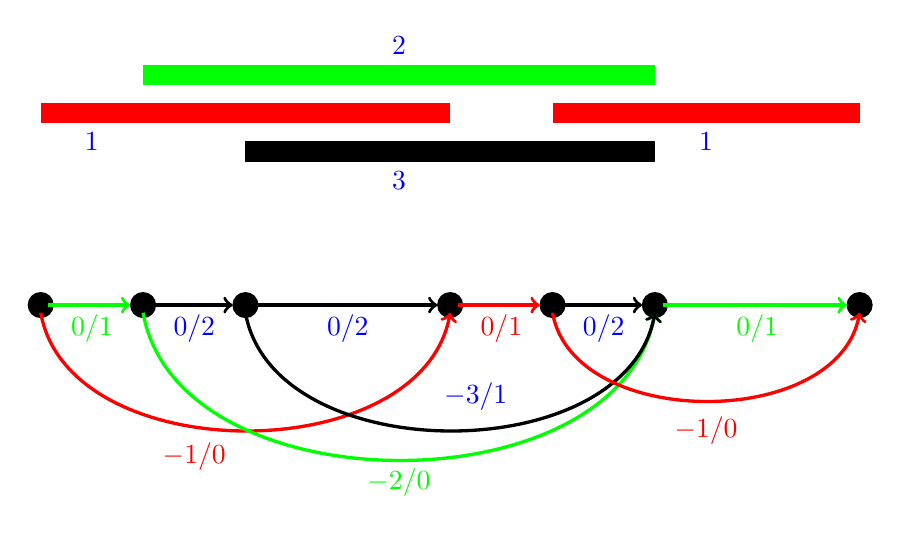
\begin{tikzpicture}[scale=0.65]

\fill[color=red] (0,0.55) rectangle (8,0.95);
\draw (1, 0.55) node[below]{\textcolor{blue}{$1$}};

\fill[color=green] (2,1.3) rectangle (12,1.7);
\draw (7, 1.7) node[above]{\textcolor{blue}{$2$}};

\fill (4,-0.2) rectangle (12,0.2);
\draw (7, -0.2) node[below]{\textcolor{blue}{$3$}};

\fill[color=red] (10,0.55) rectangle (16,0.95);
\draw (13, 0.55) node[below]{\textcolor{blue}{$1$}};

      \foreach \x in {0,2,4,8,10,12,16}
        {\draw (\x,-3) node[fill,circle] {};}


        \draw[->,very thick,color=green] (0.15,-3) -- (1.75,-3);
        \draw (1, -3) node[below]{\textcolor{green}{$0/1$}};
        \draw[->,very thick,] (2.15,-3) -- (3.75,-3);
        \draw (3, -3) node[below]{\textcolor{blue}{$0/2$}};
        \draw[->,very thick] (4.15,-3) -- (7.75,-3);
        \draw (6, -3) node[below]{\textcolor{blue}{$0/2$}};
        \draw[->,very thick,color=red] (8.15,-3) -- (9.75,-3);
        \draw (9, -3) node[below]{\textcolor{red}{$0/1$}};
        \draw[->,very thick] (10.15,-3) -- (11.75,-3);
        \draw (11, -3) node[below]{\textcolor{blue}{$0/2$}};
        \draw[->,very thick,green] (12.15,-3) -- (15.75,-3);
        \draw (14, -3) node[below]{\textcolor{green}{$0/1$}};
        
        
        \draw[->,very thick,color=red] (0,-3.15) to[out=280, in=260] (8,-3.15);
        \draw (3,-5.5) node[below] {\textcolor{red}{$-1/0$}};
        \draw[->,very thick,color=green] (2,-3.15) to[out=280, in=260] (12,-3.15);
        \draw (7,-6) node[below] {\textcolor{green}{$-2/0$}};
        \draw[->,very thick] (4,-3.15) to[out=280, in=260] (12,-3.15);
        \draw (8.5,-5.25) node[above] {\textcolor{blue}{$-3/1$}};
        \draw[->,very thick,color=red] (10,-3.15) to[out=280, in=260] (16,-3.15);
        \draw (13,-5) node[below] {\textcolor{red}{$-1/0$}};
\end{tikzpicture}
}

\end{overlayarea}

\end{frame}